\documentclass[12pt]{article}

\usepackage[spanish]{babel}
\selectlanguage{spanish}
\usepackage[utf8]{inputenc}
\usepackage{vmargin}
\usepackage{graphicx}
\setmargins{2.5cm}{1.5cm}{16.5cm}{23.42cm}{0pt}{1cm}{0pt}{2cm}

\title{Tiro Parabólico}
\author{Martín Alejandro Paredes Sosa}
\date{Abril 2015}
\graphicspath{{IMG/}}

\begin{document}
\maketitle

\section{Introducción}
En la realización de esta práctica, se estudió el tiro parabólico. Utilizando las ecuaciones de movimiento para tiro parabólico, se realizó un programa en FORTRAN, donde el usuario ingresa la velocidad inicial y ángulo de tiro, con los cuales nos permite calcular la posición en diferentes tiempos, su alcance, altura máxima y el tiempo total de vuelo.

\section{Código}
En este apartado se mostrara el código FORTRAN y la manera en que funciona.
\subsection{Algoritmo}
El programa consiste:
	\begin{enumerate}
	\item Ingreso de datos por usuario: Ángulo y velocidad del proyectil
	\item El ángulo es convertido a radianes, con el cual se descompone la velocidad en $x$ y $y$.
	\item Se crea un documento $proyectil.dat$ donde se escribirá la posición del proyectil en cada instante de tiempo $t$.
	\item Se inicia un ciclo donde se calcula la posición en ambos ejes coordenados, los cuales de escriben en $proyectil.dat$ en forma de tabla.
	\item Cuando la altura llega a 0 se termina el ciclo y se calcula el alcance y altura máxima.
	\item Se imprimen resultados en pantalla de alcance, altura máxima y tiempo total de vuelo.
\end{enumerate}
\pagebreak
\subsection{Código FORTRAN}
\begin{verbatim}
!=============================================================
!Este programa te permitira graficar el movimeinto 
!de un proyectil en un sistema ideal
!Calcula "x" y "y" en intervalos de tiempo de 0.01 segundos
!=============================================================

subroutine posicionx(v,radian,j,m,n,vx,vy,ti)
  implicit none
  Real, parameter:: g = 9.81
  Real:: m 
  Real:: n
  Real:: vx
  Real:: vy
  Real:: v, radian, ti
  integer:: j

  ti= (float(j)*0.01)
  vx= v*cos(radian)
  vy= v*sin(radian)
  m = vx*ti
  n = vy*ti-0.5*g*ti*ti
end subroutine posicionx

program proyectil
  implicit none
  !Declaración de constantes
  real , parameter :: pi=4.0*atan(1.0)
  integer, parameter :: ntps =3000
  real :: iv , rad , t , a, x, y, vx, vy, xmax, ymax
  real , parameter:: g=9.81 !gravedad
  real :: S(ntps), R(ntps)
  integer :: i
  !pi es pi y g es la gravedad
  !iv  Velocidad inicial
  !rad Angulo en radianes y "a" es el Angulo en grados
  !t Tiempo
  !"x" y "y" Donde se organizara la informacion de salida
  
  !Ingreso de datos por usuario
  write(*,*) 'Ingrese el angulo de lanzamiento en grados (Valores Reales)'
  read *, a
  write(*,*) 'Ingrese la velocidad inicial (Valores Reales)'
  read *, iv
  !transformar angulo a radianes

  rad = (a*pi)/180.0

  !Abrir archivo de salida de datos
  open (1,file='proyectil.dat')
 
 do i=1,ntps
    call posicionx(iv, rad, i, x, y,vx,vy,t)
     
    if (a==90) then
	S(i)=0 !Un tiro en 90 grados no posee movimiento 
	!en x ya que vx tiene que ser 0 (vx=v*cos(90)=0)
     else if(a==0) then
        S(i)=0 !No existe movimiento en este caso tiro de 0
        t=0
     else
	S(i)= x
     end if
     R(i)= y
     !escribir en proyectil.dat
     write(1,*) S(i), R(i)
     !Forzar salida para casos especiales cuando y es menor que 0
     if (R(i)<0) exit
  end do
  close(1)
  !Se cerro el archivo

  ymax= (vy*vy)/(2*g)
  xmax= x
    
  print *, '==========================================='
  print *, 'Velocidad inicial:', iv, 'm/s'
  print *, 'Angulo de tiro:', a, 'grados'
  print *, 'Tiempo total de vuelo', t , 's'
  print *, 'La altura maxima:', ymax, 'm'
  print *, 'Alcance del tiro:' , xmax, 'm'
  print *, '==========================================='
end program proyectil
\end{verbatim}
\pagebreak
\section{Resultados}
En este apartado se mostrara los resultados obtenidos por el .
\subsection{Tiro 0 Grados}
\begin{center}
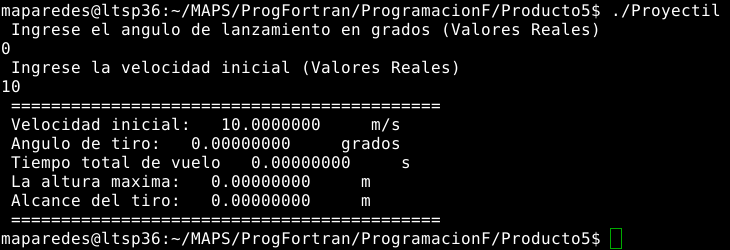
\includegraphics[width=15cm]{T0.png}
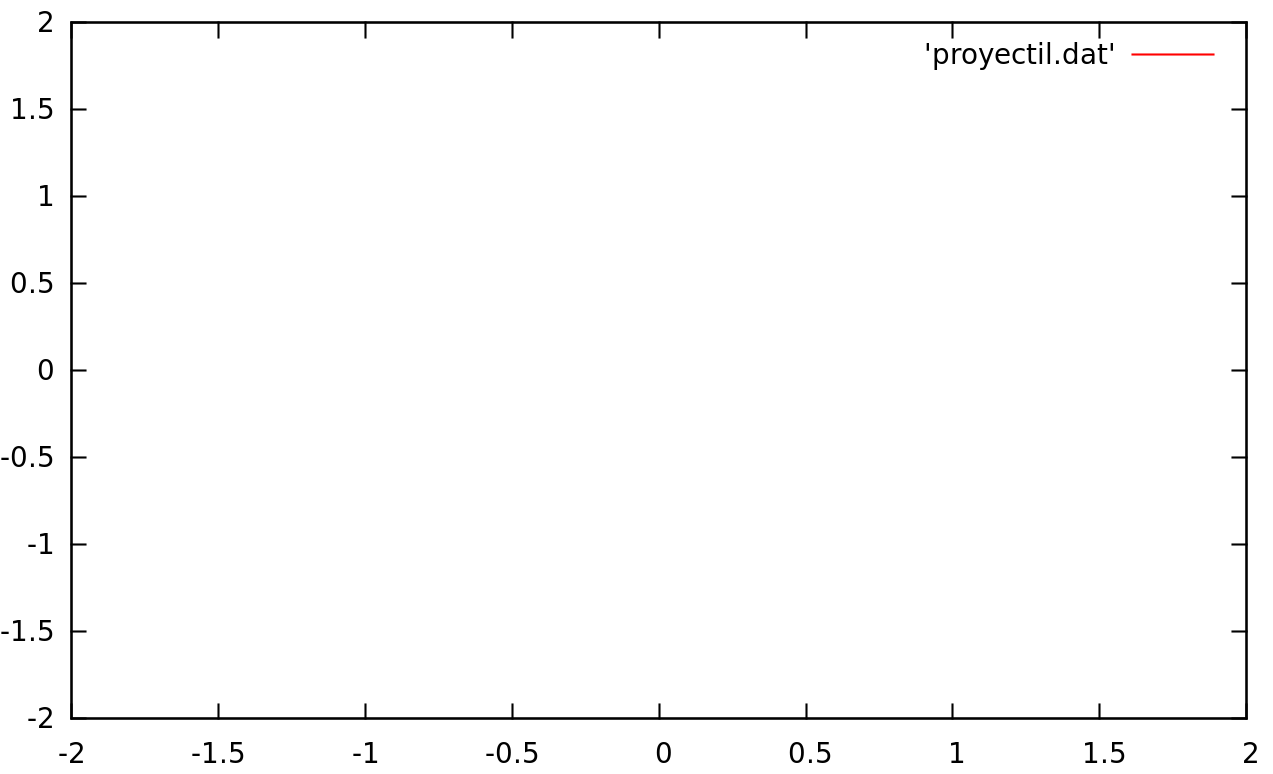
\includegraphics[width=15cm]{Parabolico0.png}
\end{center}
\subsection{Tiro 30 Grados}
\begin{center}
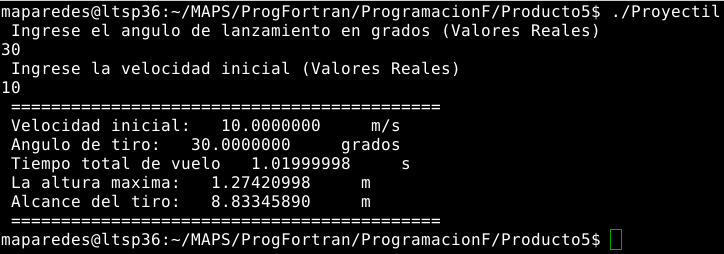
\includegraphics[width=15cm]{T30.png}
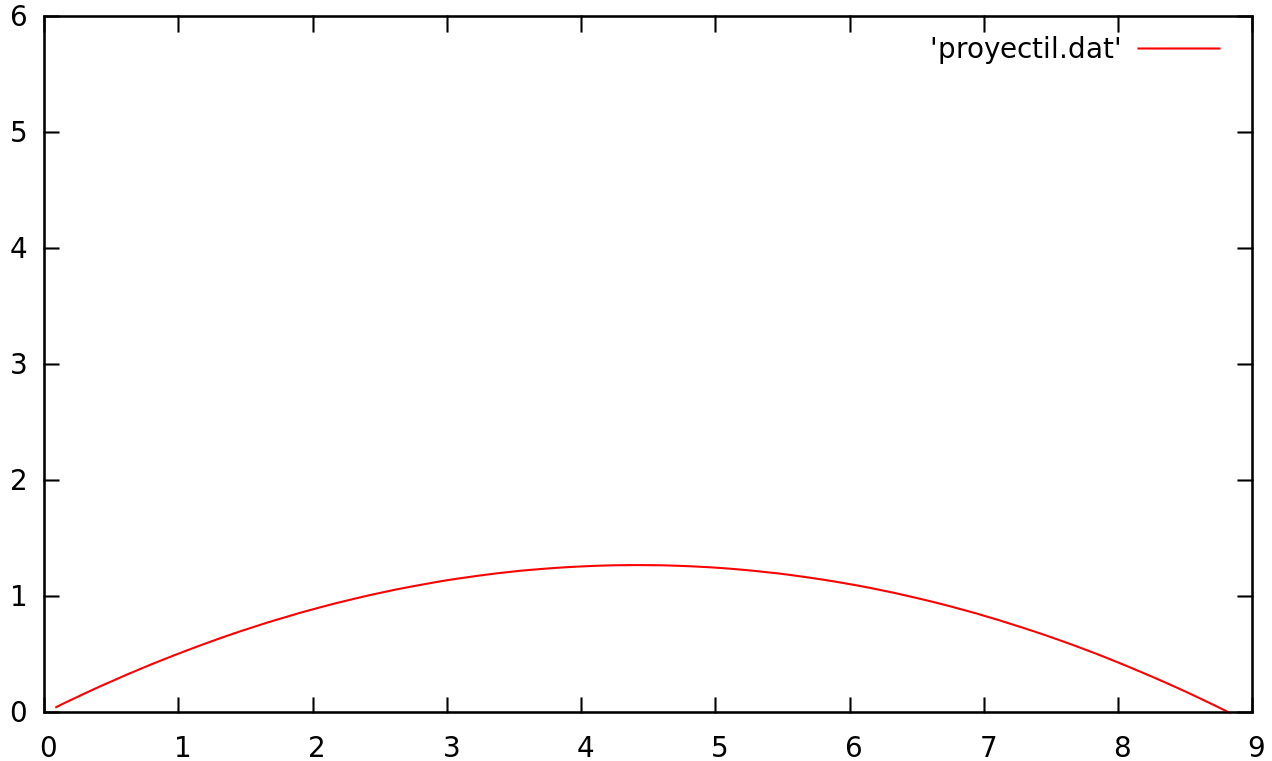
\includegraphics[width=15cm]{Parabolico30.png}
\end{center}
\subsection{Tiro 60 Grados}
\begin{center}
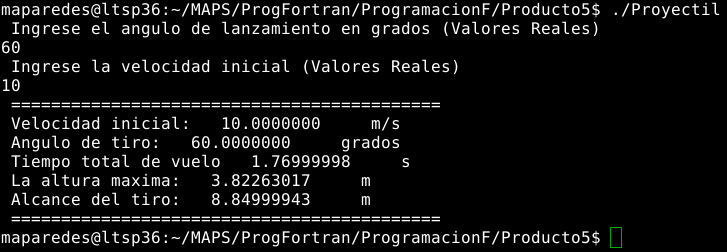
\includegraphics[width=15cm]{T60.png}
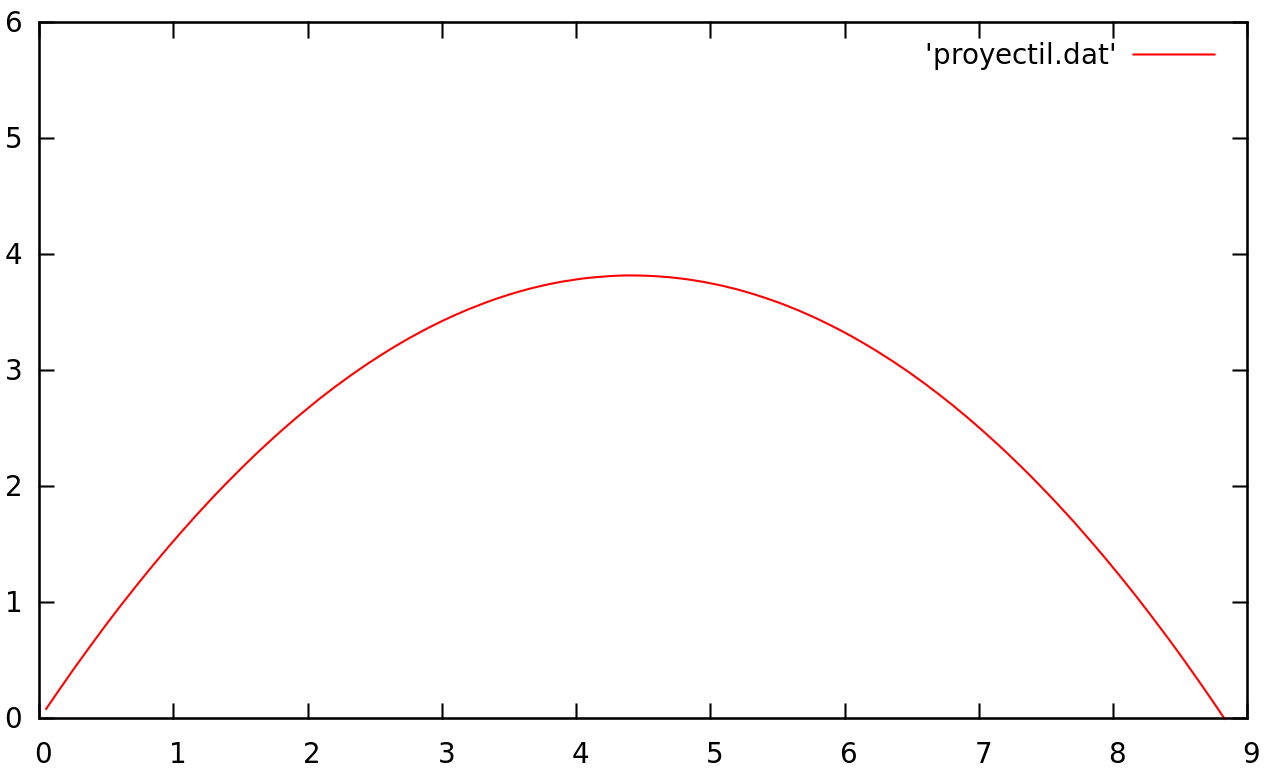
\includegraphics[width=15cm]{Parabolico60.png}
\end{center}
\subsection{Tiro 90 Grados}
\begin{center}
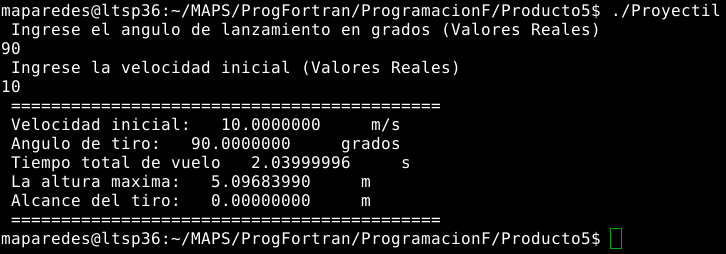
\includegraphics[width=15cm]{T90.png}
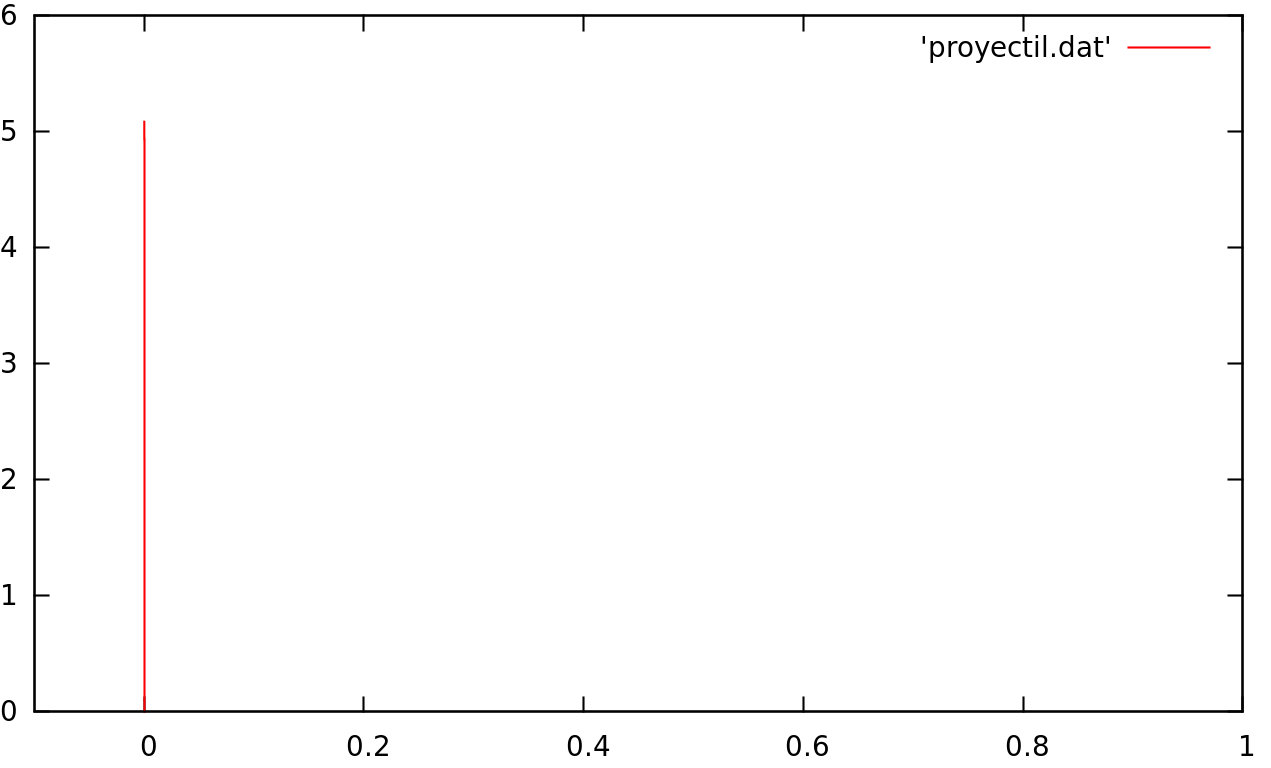
\includegraphics[width=15cm]{Parabolico90.png}
\end{center}
\end{document}
